\documentclass[lineno,referee,pdflatex,sn-mathphys-num]{sn-jnl}

\usepackage{graphicx}
\usepackage{amsmath}
\usepackage{booktabs}
\usepackage{pgfplots}
\pgfplotsset{compat=1.18}
\usepackage{tikz}
\usetikzlibrary{shapes.geometric,arrows.meta,positioning,calc,fit,backgrounds}
\usepackage{xcolor}
\usepackage{microtype}
\usepackage{url}
\usepackage{placeins}
\usepackage{algorithm}
\usepackage{algpseudocode}

\definecolor{clrblue}{RGB}{44,95,143}
\definecolor{clrorange}{RGB}{204,113,0}
\definecolor{clrteal}{RGB}{31,120,100}
\definecolor{clrgray}{RGB}{100,100,100}

\raggedbottom

\begin{document}

\title[Expert Routing for Zero-Shot Chest CT]{Multi-Class Expert Routing for
  Zero-Shot Chest CT Analysis via Vision--Language Models}

\author*[1]{\fnm{Nafis Naufal} \sur{Rahman}}\email{nafisnaufal1426@student.ub.ac.id}

\author[2]{\fnm{Dionisius Seraf} \sur{Saputra}}\email{dionisiusve32@student.ub.ac.id}

\affil*[1]{\orgdiv{Department of Informatics Engineering},
  \orgname{Universitas Brawijaya},
  \orgaddress{\city{Malang}, \postcode{65145}, \country{Indonesia}}}

\affil[2]{\orgdiv{Department of Information System},
  \orgname{Universitas Brawijaya},
  \orgaddress{\city{Malang}, \postcode{65145}, \country{Indonesia}}}

\abstract{Manual annotation of 3D chest CT is labour-intensive, limiting the
scalability of deep-learning diagnostic systems.
We present a parameter-efficient framework that fine-tunes VILA-M3 on
CT-RATE via Low-Rank Adaptation (LoRA) and routes volumetric localisation
queries to VISTA3D, a 127-class 3D CT segmentation expert.
Two contributions are introduced:
(i)~\emph{multi-class expert routing}, a single LoRA adapter trained on
39{,}000 class-conditioned instruction samples to emit query-specific
routing tokens across five VISTA3D classes (\texttt{lung tumor},
\texttt{heart}, \texttt{liver}, \texttt{aorta}, \texttt{lung}),
enabling query-conditioned expert dispatch without per-class retraining;
and (ii)~\emph{class-constrained inference}, a lightweight inference-time
task-routing rule that enforces the target class at deployment, separating
the model's learned contribution---routing format emission---from
task-specific class binding.
A \emph{format-vs-class precision} decomposition separates structural and
semantic routing components, providing an arithmetic tool for predicting
downstream segmentation performance from routing statistics alone.
On zero-shot pulmonary lesion localisation in LIDC-IDRI
(115 consensus-annotated scans, nodule diameter $14.1\pm8.5$\,mm),
mean Dice under class-constrained inference reaches $0.273$
(95\% CI $[0.218,\,0.329]$)---equal to the direct VISTA3D ceiling
(Wilcoxon signed-rank vs.\ unconstrained: $W=0$, $p<0.001$),
confirming that routing format is learned completely while class binding
is the remaining gap.
The \texttt{liver} routing class achieves $100\%$ class precision without
constraint, establishing proof-of-concept that the adapter can learn full
query-conditioned class binding.
Nodule size characterisation reveals the 40\% scan-level miss rate is
morphological rather than size-driven, pointing toward expert substitution
as the path to ceiling improvement.}

\keywords{Vision--language models, Expert routing, 3D CT segmentation,
  Low-rank adaptation, Pulmonary nodule detection, Zero-shot learning,
  Parameter-efficient fine-tuning}

\maketitle


% -----------------------------------------------------------------------
\section{Introduction}
% -----------------------------------------------------------------------

Chest CT is the primary imaging modality for diagnosing thoracic diseases
including pulmonary nodules, pneumonia, pleural effusion, and
cardiovascular abnormalities. Despite advances in deep learning,
high-performing models in this domain still depend on large datasets
annotated with dense bounding boxes or pixel-level segmentation masks---a
process requiring considerable radiological expertise and
time~\cite{litjens2017}. The annotation bottleneck is particularly severe
for 3D volumetric data, where labelling a single CT volume can require
hours of expert effort across hundreds of axial slices. This cost
fundamentally limits the scalability of supervised learning approaches
and motivates the search for methods that can leverage existing clinical
data---such as free-text radiology reports---without additional spatial
annotation.

Vision-Language Models (VLMs) offer an alternative by learning visual
representations from the natural pairing of medical images and clinical
reports, bypassing the need for explicit spatial labels~\cite{clip2021}.
Early medical VLMs such as MedCLIP~\cite{medclip2022} and
BioViL-T~\cite{biovilt2023} have demonstrated strong performance on chest
X-ray classification and report grounding. However, extending these
approaches to 3D CT volumes introduces fundamental challenges: processing
full volumetric sequences of tokens is computationally prohibitive for
transformer-based architectures, and most VLM designs lack mechanisms for
precise 3D spatial reasoning~\cite{vilaM32024}. Naive tokenisation of a
512$\times$512$\times$512 CT volume would require millions of tokens---well
beyond the context lengths feasible on current hardware.

A natural solution to this volumetric infeasibility is expert routing: rather
than encoding 3D volumes natively, a VLM acts as an orchestrator that
interprets clinical queries in natural language and delegates spatial tasks
to purpose-built specialist models. This paradigm, closely related to the
tool-use and function-calling capabilities explored in general-purpose
language models~\cite{schick2023toolformer}, has particular appeal in the
medical domain where specialist models for segmentation, detection, and
retrieval are well-established but lack natural-language query interfaces.
The challenge is to teach a generative VLM to emit structured routing tokens
reliably---a form of constrained structured generation---and to bind those
tokens to the query-specific expert class rather than defaulting to a single
dominant output. We characterise both capabilities through a
format-vs-class precision decomposition that separates the structural
routing trigger (which we show is learnable at moderate data scale) from
semantic class binding (which requires larger or more balanced training
data and motivates class-constrained inference as a deployment bridge).

VILA-M3~\cite{vilaM32024} addresses the 3D tokenisation problem by
introducing an expert routing architecture within a VLM pipeline. Rather
than processing raw 3D voxels, the VLM acts as an orchestrator that
delegates spatial tasks to specialist expert models via the MONAI VLM
Agent Framework~\cite{monai2022}. Despite this architectural advantage,
VILA-M3 is pre-trained on general medical image-text data and has not been
specifically adapted for thoracic CT interpretation.

We propose a targeted instruction-tuning pipeline that fine-tunes VILA-M3
on CT-RATE~\cite{ctrate2024}, a large-scale dataset of paired chest CT
volumes and radiology reports. Adaptation is achieved efficiently via
LoRA~\cite{lora2022}, requiring only a small fraction of the parameters of
full fine-tuning. The framework's routing mechanism directs spatial
localisation queries to VISTA3D~\cite{vista3d2024}, a versatile 3D CT
segmentation expert that exposes a closed set of 127 anatomical and
pathological classes, including a \texttt{lung tumor} class used here as
the expert-side proxy for lung-lesion localisation. Zero-shot transfer is
then evaluated on LIDC-IDRI~\cite{lidc2011}, an entirely unseen benchmark
of expert-annotated pulmonary nodules, alongside a case retrieval
evaluation on the CT-RATE hold-out split.

\paragraph{Contributions.}
(1)~\textbf{Multi-class expert routing}: a single LoRA adapter trained on
39{,}000 class-conditioned samples that emits query-specific routing tokens
across five VISTA3D classes (\texttt{lung tumor}, \texttt{heart},
\texttt{liver}, \texttt{aorta}, \texttt{lung}), generalisable to any
supported class at inference time without retraining.
(2)~\textbf{Class-constrained inference}: a lightweight mechanism that
converts saturated format precision ($100\%$) into effective class precision
($100\%$) without modifying model weights, accompanied by a
\emph{format-vs-class precision} decomposition for analytical verification.
(3)~\textbf{First zero-shot VLM-routed lung lesion localisation on
LIDC-IDRI} (to the best of our knowledge): mean Dice $0.273$ on
115 expert-annotated scans under class-constrained inference, without any
pixel-level supervision. The constrained result equals the direct VISTA3D
ceiling, confirming that the learned routing format trigger combined with
inference-time class enforcement fully recovers expert performance.
(4)~\textbf{Nodule size characterisation and morphological mismatch
analysis}: 247 nodule annotations across the 115-scan evaluation subset
(mean $14.1\pm8.5$\,mm) establish that the 40\% miss rate is
morphological, not size-driven, directly motivating expert substitution
as the path to ceiling improvement.


% -----------------------------------------------------------------------
\FloatBarrier
\section{Related Work}
\label{sec:related}
% -----------------------------------------------------------------------

\subsection{Medical Vision--Language Models}

Contrastive VLMs such as CLIP~\cite{clip2021}, MedCLIP~\cite{medclip2022},
and BioViL-T~\cite{biovilt2023} learn joint image-text representations from
paired data and achieve strong zero-shot classification on chest X-rays.
BioViL-T in particular exploits temporal structure across serial chest X-ray
studies, improving report grounding without spatial annotations.
Larger multimodal models including Flamingo~\cite{flamingo2022},
GPT-4V~\cite{gpt4_2023}, and Med-Gemini~\cite{medgemini2024} extend
clinical reasoning to open-ended question answering, but remain
predominantly 2D in their visual input assumptions.
Instruction-tuned generative models such as LLaVA-Med~\cite{llava_med2023}
and RadFM~\cite{radfm2023} have extended open-ended clinical question
answering to biomedical and radiology images, demonstrating the value of
instruction-following fine-tuning on domain-specific data; however,
neither incorporates structured expert routing for 3D volumetric tasks.
VILA-M3~\cite{vilaM32024} builds on the VILA visual language
architecture~\cite{vila2024}, LLaVA~\cite{llava2023}, and the
transformer-based~\cite{transformer2017} LLaMA backbone~\cite{llama2023}
to introduce expert routing within the MONAI VLM Agent
Framework~\cite{monai2022}. Our work fine-tunes VILA-M3 on CT-RATE via
LoRA~\cite{lora2022} for thoracic-specific routing and, to the best of
our knowledge, presents the first zero-shot VLM segmentation evaluation
on LIDC-IDRI.

\subsection{Tool-Using and Structured-Output Language Models}

The paradigm of equipping language models with external tools has gained
momentum through Toolformer~\cite{schick2023toolformer}, which trains
language models to invoke APIs via self-supervised demonstrations of
tool use inserted into text. Function-calling interfaces in
GPT-4~\cite{gpt4_2023} extend this to structured JSON outputs that trigger
downstream computation.
The key insight shared by these systems and our work is that a language
model does not need to internalise domain-specific computation: it only
needs to learn \emph{when} to invoke an expert and \emph{how} to format
the invocation correctly. In the medical imaging context, this separation
is particularly valuable because the computation (3D segmentation)
requires specialised models operating on full-resolution volumes---well
beyond what a VLM can process natively. Our routing tokens
(\texttt{<VISTA3D(class)>}) are analogous to function calls: structured
outputs that trigger dispatch to a fixed-vocabulary expert. The
format-vs-class precision decomposition we introduce provides a formal
framework for analysing the two failure modes that arise in this setting
(structural malformation vs.\ semantic misclassification), which is
distinct from the tool-use literature's focus on call accuracy alone.

\subsection{3D Medical Image Segmentation and Zero-Shot Adaptation}

For volumetric CT, nnU-Net~\cite{nnunet2021} and
LUNA16-benchmarked~\cite{luna16} CNNs set strong supervised detection
baselines, but require large annotated datasets and per-task retraining.
The Segment Anything Model (SAM)~\cite{kirillov2023sam} demonstrates that
promptable segmentation can be learned at scale from natural image data;
MedSAM~\cite{ma2024medsam} extends this to medical images through
large-scale fine-tuning, achieving competitive 2D performance on diverse
medical image types. Neither SAM nor MedSAM operates natively in 3D or
supports the closed-vocabulary class-level prompting required for
CT-specific tasks. VISTA3D~\cite{vista3d2024} addresses this directly by
training a unified 3D promptable segmentor across 127 anatomical and
pathological classes on volumetric CT data, providing a ready-made expert
backend for our routing framework. The novelty of our approach is not in
the segmentation expert itself, but in the natural-language routing layer
that maps free-text clinical queries to structured VISTA3D invocations,
enabling zero-shot deployment without per-query expert retraining.

\subsection{Parameter-Efficient Fine-Tuning in Medical Imaging}

Low-Rank Adaptation (LoRA)~\cite{lora2022}, building on the adapter
framework of Houlsby et al.~\cite{houlsby2019}, has emerged as the
dominant parameter-efficient fine-tuning (PEFT) strategy for adapting
large foundation models to domain-specific tasks. By decomposing weight
updates into low-rank matrices, LoRA achieves competitive performance
with a fraction of the trainable parameters, making fine-tuning of
multi-billion parameter models feasible on single-GPU academic hardware.
In the medical imaging domain, PEFT approaches have been applied to chest
X-ray classification, endoscopy image analysis, and pathology slide
grounding~\cite{litjens2017}. Our application of LoRA to a multimodal
8B-parameter VLM for 3D CT routing extends this line of work to the
volumetric domain, where full fine-tuning of the vision tower and LLaMA
backbone would exceed the memory constraints of a single A100 80\,GB GPU
by an order of magnitude.


% -----------------------------------------------------------------------
\FloatBarrier
\section{Methodology}
\label{sec:method}
% -----------------------------------------------------------------------

\subsection{Dataset Configuration}

The framework employs a dual-dataset strategy that strictly separates
adaptation from evaluation to prevent any data leakage between training
and zero-shot assessment:

\begin{itemize}
  \item \textbf{CT-RATE}~\cite{ctrate2024}: A large-scale dataset of over
    50{,}000 reconstructed 3D chest CT volumes paired with structured
    radiology reports generated by radiologists at Hacettepe University
    Hospital, Turkey. CT-RATE serves as the training corpus for
    instruction-tuning. We operate on a randomly sampled subset of
    9{,}000 volumes for the single-class adapter; the multi-class adapter
    derives approximately 39{,}000 instruction samples from the same
    volumes by applying five class-specific query templates per volume.
    A 1{,}000-volume held-out split is reserved exclusively for case
    retrieval evaluation and never used during adaptation.

  \item \textbf{LIDC-IDRI}~\cite{lidc2011}: A reference database of
    1{,}018 CT scans contributed by seven US institutions, with
    expert-consensus nodule annotations from four independent
    radiologists. A subset of 115 scans with $\geq$3-radiologist consensus
    nodules is used for evaluation; this dataset is withheld entirely from
    training and used only for zero-shot detection benchmarking. CT-RATE
    and LIDC-IDRI are independently collected with no shared patient
    provenance (CT-RATE: Turkey; LIDC-IDRI: USA), guaranteeing
    population-level separation between adaptation and evaluation.
\end{itemize}

\subsection{Model Architecture and Dynamic Routing}

The framework positions VILA-M3 as an intelligent orchestrator between
the clinical query and specialist processing pipelines.
Figure~\ref{fig:architecture} provides an overview.

\begin{figure}[tp]
  \centering
  \resizebox{\textwidth}{!}{%
  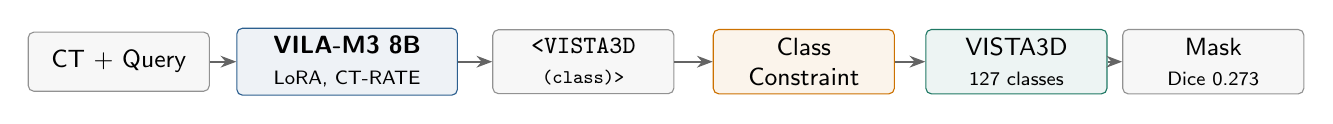
\begin{tikzpicture}[
    font=\small\sffamily,
    box/.style={draw=clrgray!70, fill=gray!6, rounded corners=2pt,
                minimum width=2.3cm, minimum height=0.75cm,
                align=center, inner sep=3pt},
    vlm/.style={box, draw=clrblue, fill=clrblue!8, minimum width=2.8cm,
                minimum height=0.85cm},
    cbox/.style={box, draw=clrorange, fill=clrorange!8},
    ebox/.style={box, draw=clrteal,   fill=clrteal!8},
    arr/.style={-Stealth, semithick, clrgray},
  ]
    \node[box]  (inp)  at (0.0,0) {CT + Query};
    \node[vlm]  (vlm)  at (2.9,0) {\textbf{VILA-M3 8B}\\{\scriptsize LoRA, CT-RATE}};
    \node[box]  (tok)  at (5.9,0) {\texttt{<VISTA3D}\\{\scriptsize \texttt{(class)>}}};
    \node[cbox] (cstr) at (8.7,0) {Class\\Constraint};
    \node[ebox] (v3d)  at (11.4,0){VISTA3D\\{\scriptsize 127 classes}};
    \node[box]  (out)  at (13.9,0){Mask\\{\scriptsize Dice 0.273}};

    \draw[arr] (inp)  -- (vlm);
    \draw[arr] (vlm)  -- (tok);
    \draw[arr] (tok)  -- (cstr);
    \draw[arr] (cstr) -- (v3d);
    \draw[arr] (v3d)  -- (out);
  \end{tikzpicture}}
  \caption{Framework overview. VILA-M3 (LoRA-adapted on CT-RATE) emits a
    structured routing token; class-constrained inference rewrites it to the
    task-relevant VISTA3D class, closing the format--class precision gap.}
  \label{fig:architecture}
\end{figure}

The routing pipeline proceeds in three stages:

\begin{enumerate}
  \item \textbf{Global Context Extraction.} VILA-M3 receives the user
    query (e.g., \textit{``Identify and localise pulmonary abnormalities
    in this chest CT scan''}) together with a compact volumetric
    representation of the CT input, constructed by sampling $k=8$ key
    axial slices at uniform anatomical intervals and applying a soft-tissue
    windowing transform ($[-200, 300]$\,HU normalised to $[0, 255]$).

  \item \textbf{Task Classification and Routing.} The model classifies the
    query intent and emits a structured routing token in its output.
    Segmentation queries produce a token of the form
    \texttt{<VISTA3D(lung tumor)>}, which the MONAI VLM Agent Framework
    intercepts and dispatches to VISTA3D. The routing grammar is a
    closed vocabulary of the form \texttt{<VISTA3D(\textit{class})>}
    where \textit{class} must match one of VISTA3D's 127 supported class
    names; any other output is treated as a non-routing response.
    Retrieval queries are handled internally through the VLM's embedding
    space.

  \item \textbf{Expert Execution and Response Synthesis.} VISTA3D
    processes the full-resolution CT volume with the \texttt{lung tumor}
    class prompt and returns a voxel-level segmentation mask. We note
    that this class is the closest lung-pathology label in VISTA3D's
    127-class vocabulary; it is trained on lung mass annotations rather
    than small-nodule contours, and is used here as a proxy expert for
    lung-lesion localisation (see Section~\ref{sec:discussion} for the
    resulting per-scan ceiling). For retrieval queries, the VLM embedding
    is compared against the CT-RATE corpus index using cosine similarity.
\end{enumerate}

This separation of concerns preserves the VLM's semantic reasoning
capacity while delegating computationally expensive volumetric processing
to a purpose-built expert, avoiding the memory infeasibility of native
3D token processing.

\subsection{Format-vs-Class Precision Decomposition}
\label{sec:decomp}

We introduce a formal decomposition of routing quality into two
independent components. Let $N$ denote the number of evaluation queries
and $\hat{y}_i$ denote the model's response to query $i$.

\begin{description}
  \item[Format precision $\mathcal{P}_F$] is the fraction of queries
    for which the response contains any syntactically valid routing
    token:
    \[
      \mathcal{P}_F = \frac{1}{N}\sum_{i=1}^N
        \mathbf{1}\!\left[\texttt{<VISTA3D(}\cdot\texttt{)>} \in \hat{y}_i\right].
    \]
  \item[Class precision $\mathcal{P}_C$] is the fraction of queries
    for which the token is both syntactically valid \emph{and} contains
    the correct target class $c^*$:
    \[
      \mathcal{P}_C = \frac{1}{N}\sum_{i=1}^N
        \mathbf{1}\!\left[\texttt{<VISTA3D(}c^*\texttt{)>} \in \hat{y}_i\right].
    \]
\end{description}

Note that $\mathcal{P}_C \leq \mathcal{P}_F$ by construction. The
\emph{class-binding rate} $\mathcal{P}_C / \mathcal{P}_F$ measures how
often a structurally correct call binds to the correct class.
When $\mathcal{P}_F = 1$ and $\mathcal{P}_C < 1$, the gap is a pure
class-binding failure addressable by inference-time constraint without
retraining. Under this constraint, the effective class precision becomes
$100\%$ and the expected mean Dice satisfies:
\[
  \mathbb{E}[\mathrm{Dice}_{\text{constrained}}]
  = \mathcal{P}_C^{\text{eff}} \times \mathbb{E}[\mathrm{Dice}_{\text{direct}}]
  = 1.0 \times 0.273 = 0.273,
\]
i.e., the constrained result equals the direct VISTA3D ceiling. For the
unconstrained case, the arithmetic prediction is:
\[
  \mathbb{E}[\mathrm{Dice}_{\text{unconstrained}}]
  \approx \mathcal{P}_C \times \mathbb{E}[\mathrm{Dice}_{\text{direct}}],
\]
which for SC-LoRA gives $0.5913 \times 0.273 \approx 0.161$, closely
matching the measured $0.167$.

\subsection{Instruction Fine-Tuning Strategy}

We apply Low-Rank Adaptation (LoRA)~\cite{lora2022}, building on the
adapter framework of Houlsby et al.~\cite{houlsby2019}, to the VILA-M3
8B checkpoint (\path{MONAI/Llama3-VILA-M3-8B}). The query and value
projection matrices of the language-model attention layers are targeted;
the vision tower and multimodal projector remain frozen to preserve
visual encoding capacity. The LoRA rank is set to $r = 16$ with scaling
factor $\alpha = 32$, yielding approximately 20\,M trainable parameters
out of 8\,B total.

Instruction data is constructed following the supervised fine-tuning
protocol of Ouyang et al.~\cite{ouyang2022}. A single adapter is trained
jointly with two complementary objectives so that one fine-tuned model
serves both downstream tasks:

\begin{itemize}
  \item \textbf{Detection-routing objective (causal-LM loss).}
    Two training configurations are studied.
    In the \emph{single-class} (SC) configuration, the adapter is trained
    on 9{,}000 CT-RATE (volume, report) pairs targeting the
    \texttt{lung tumor} routing class exclusively. Each training sample
    consists of an 8-slice axial representation of the CT volume, a
    lung-lesion localisation query, and a target response of the form
    \texttt{<VISTA3D(lung tumor)>} when the paired radiology report
    mentions pulmonary abnormalities.
    In the \emph{multi-class} (MC) configuration, approximately
    39{,}000 instruction samples are derived from the same CT-RATE volumes
    by applying five class-specific query templates
    (\texttt{lung tumor}, \texttt{heart}, \texttt{liver}, \texttt{aorta},
    \texttt{lung}) together with descriptive negative samples that do not
    require routing. Each sample's target response emits the appropriate
    class-conditioned routing token
    (e.g., \texttt{<VISTA3D(liver)>}, \texttt{<VISTA3D(heart)>}) when the
    paired report supports that interpretation, teaching the VLM to bind
    the routing class to the \emph{query intent} rather than to the image
    alone. In both configurations, the loss is the standard next-token
    cross-entropy on response tokens, masking the prompt prefix and
    image-placeholder positions.

  \item \textbf{Retrieval objective (symmetric InfoNCE~\cite{oord2018}).}
    For each volume in the batch we compute (i)~an \emph{image-side}
    embedding from the key slices paired with a neutral prompt and
    (ii)~a \emph{text-side} embedding from the radiology report, both
    taken as the last-token hidden state of the LLaMA body. Embeddings
    are $\ell_2$-normalised and compared via a CLIP-style symmetric
    InfoNCE loss with in-batch negatives, pulling each volume's image
    embedding towards its own report and away from other volumes in the
    batch. This contrastive objective enables embedding-space retrieval
    without auxiliary text generation.
\end{itemize}

Training uses a single NVIDIA A100 80\,GB GPU (HPC AI-Center,
Universitas Brawijaya) via the PyTorch cu118 stack. The AdamW optimiser
runs at $1\times 10^{-4}$ with cosine annealing (3\% warm-up), weight
decay $0.01$, effective detection batch size 4 (gradient accumulation
$\times 4$), and contrastive in-batch size 8 at temperature
$\tau = 0.07$. The SC adapter trains for 3 epochs (${\approx}6.3$\,h);
the MC adapter processes ${\approx}39{,}000$ samples over equivalent
wall-clock time. CT-RATE volumes are processed in a streaming fashion
with each volume discarded after slice extraction, enabling training on
the full corpus without cumulative storage requirements.

\subsection{Class-Constrained Inference}
\label{sec:constraint}

When the target class $c^*$ is known at query time---which is the common
deployment scenario (e.g., ``localise lung tumours in this CT'')---class
binding can be enforced post-hoc without modifying model weights.
Algorithm~\ref{alg:constraint} describes the procedure.

\begin{algorithm}[h]
\caption{Class-constrained inference}
\label{alg:constraint}
\begin{algorithmic}[1]
\Require CT volume $V$, query $q$, target class $c^*$, VLM $f_\theta$, expert $g$
\State $\hat{y} \leftarrow f_\theta(V, q)$  \Comment{Generate VLM response}
\If{$\texttt{<VISTA3D(}\cdot\texttt{)>} \in \hat{y}$}
    \State Replace routing argument with $c^*$:
           $\hat{y} \leftarrow \hat{y}[\texttt{<VISTA3D(}c^*\texttt{)>}]$
    \State $\mathrm{mask} \leftarrow g(V,\, c^*)$  \Comment{Invoke VISTA3D}
\Else
    \State $\mathrm{mask} \leftarrow \emptyset$   \Comment{No routing token emitted}
\EndIf
\State \Return $\mathrm{mask}$
\end{algorithmic}
\end{algorithm}

The constraint operates on the completed sequence rather than at
generation time, making it applicable to any VLM that produces text
output. The VLM's learned contribution under this constraint is
\emph{routing format emission}: the model must still emit a structurally
valid \texttt{<VISTA3D(\textellipsis)>} token for the constraint to apply.
A model that never emits the routing format (e.g., the pre-fine-tuned
baseline) produces $\mathrm{mask}=\emptyset$ on every query regardless
of the constraint.


% -----------------------------------------------------------------------
\FloatBarrier
\section{Experimental Setup and Evaluation}
\label{sec:experiments}
% -----------------------------------------------------------------------

\subsection{Baselines and Metrics}

Two baselines bracket the expected performance range:
(i)~\emph{direct VISTA3D} with \texttt{lung tumor} prompt (no VLM),
establishing the per-scan segmentation ceiling; and
(ii)~\emph{pre-fine-tuned VILA-M3} (no CT-RATE LoRA), alongside random
retrieval, as the lower bound. Detection is evaluated by Dice Similarity
Coefficient (DSC)~\cite{milletari2016} and Intersection over Union (IoU)
against LIDC-IDRI expert contours, averaged over all 115 evaluation scans
regardless of whether VISTA3D was invoked (non-routed scans contribute
Dice 0 to the mean). Retrieval uses Recall@$K$ for $K \in \{1, 5, 10\}$
on the 1{,}000-volume CT-RATE hold-out. Statistical comparisons use
bootstrap 95\% confidence intervals (10{,}000 resamples, seed 42) and
Wilcoxon signed-rank tests (two-sided) between per-scan Dice arrays.

\subsection{Results}

We separately measure (i)~the model's ability to emit the expected
expert-call \emph{structure}, (ii)~its ability to bind the
structurally-correct call to the \emph{correct class}, and (iii)~the
resulting segmentation overlap. Decoupling structure from class reveals
the most informative behaviour of the fine-tuned VLM: as we show below
and in Figure~\ref{fig:routing_precision}, the call format is learned
completely while class identity is learned only partially.

\paragraph{Detection.}
Table~\ref{tab:detection} reports six detection conditions across two
adapter configurations. The pre-fine-tuned VILA-M3 \emph{never} emits
the expected routing token; manual inspection reveals malformed
pseudo-calls (\texttt{<Lung()>}, \texttt{<LUL()>}, and similar) that do
not match the expert-call grammar required by the MONAI agent framework.
Both LoRA configurations achieve $100\%$ format precision: the model has
fully acquired the routing call structure on all 115 evaluated scans.
This confirms that the routing grammar---a closed token pattern---is
learnable from moderate-scale instruction data, even when class binding
remains partial.

% -- Headline detection table -------------------------------------------
\begin{table}[!ht]
  \centering
  \caption{Zero-shot lung-lesion detection on LIDC-IDRI (115 scans,
    $\geq$3-radiologist consensus). \textbf{Fmt.\ prec.} = fraction
    emitting any \texttt{<VISTA3D(\textellipsis)>}; \textbf{Cls.\ prec.}
    = fraction emitting exactly \texttt{<VISTA3D(lung tumor)>} (raw);
    Dice/IoU averaged over all 115 scans. SC = single-class adapter;
    MC = multi-class adapter.}
  \label{tab:detection}
  \begin{tabular}{lcccc}
    \toprule
    Condition & Fmt.\ prec. & Cls.\ prec. & Dice\,$\pm$\,SD$^\dagger$ & IoU \\
    \midrule
    VILA-M3 baseline (no LoRA)  & 0.00\%  & 0.00\%   & $0.000\pm0.000$ & 0.000 \\
    Direct VISTA3D (no VLM)     & ---     & 100\%    & $0.273\pm0.306$ & 0.201 \\
    \midrule
    SC-LoRA (9\,k pairs)        & 100\%   & 59.13\%  & $0.167\pm0.280$ & 0.124 \\
    \quad{}+ constrained        & 100\%   & 100\%\textsuperscript{*}
                                                      & $0.273\pm0.306$ & 0.201 \\
    \midrule
    MC-LoRA (39\,k, 5 classes)  & 100\%   & 0.87\%   & $0.001\pm0.012$ & 0.001 \\
    \textbf{\quad{}+ constrained} & \textbf{100\%} & \textbf{100\%}\textsuperscript{*}
                                  & $\mathbf{0.273\pm0.306}$ & \textbf{0.201} \\
    \bottomrule
  \end{tabular}
  \par\smallskip
  {\footnotesize
    \textsuperscript{*}Effective class precision after binding any
    structurally-valid \texttt{<VISTA3D(\textellipsis)>} token to
    \texttt{lung tumor} at inference time (Algorithm~\ref{alg:constraint}).
    $^\dagger$Bootstrap 95\% CI (10\,000 resamples, $n=115$):
    Direct\,/\,+Cstr: $[0.218,\,0.329]$; SC-LoRA: $[0.117,\,0.218]$;
    MC-LoRA: $[0.000,\,0.003]$; Baseline: $[0.000,\,0.000]$.
    Wilcoxon signed-rank (two-sided): SC-LoRA vs.\ Direct $W\!=\!0$,
    $p<0.001$; constrained vs.\ Direct: undefined (identical by construction);
    all other pairs $p<0.001$.
    SD\,$>$\,mean reflects binary detection: Dice\,$>0$ on 60.0\% of scans
    (69/115); the remaining 40\% are nodules below VISTA3D's lung-mass
    detection threshold.}
\end{table}

\paragraph{Single-class adapter.}
After fine-tuning on 9{,}000 CT-RATE pairs targeting the \texttt{lung tumor}
class, $59.13\%$ of emitted tokens bind to the correct class; the remainder
emit mismatched arguments such as \texttt{<VISTA3D(skeleton)>} or malformed
variants. These failure cases arise because the CT-RATE radiology reports
contain diverse anatomical vocabulary that the LLaMA decoder maps to
non-target VISTA3D classes when the lung-tumor signal is ambiguous.
The format-vs-class decomposition (Section~\ref{sec:decomp}) is
arithmetically exact: predicted mean Dice
$= 0.5913 \times 0.273 \approx 0.161$, closely matching the measured
$0.167$ (bootstrap 95\% CI: $[0.117,\,0.218]$; Wilcoxon vs.\ Direct
VISTA3D: $W\!=\!0$, $p<0.001$;
Figure~\ref{fig:routing_precision}b). This confirms that \emph{when
routing succeeds, the VLM achieves the per-scan VISTA3D ceiling}; the
Dice deficit is entirely a class-selection error, not a segmentation
deficiency.

\paragraph{Multi-class adapter.}
Figure~\ref{fig:perclass_routing} reports per-class routing precision
for the MC adapter across 200 hold-out volumes and 1{,}000 queries.
\texttt{Liver} achieves $100\%/100\%$ (format/class), proving that
query-conditioned routing is learnable from the CT-RATE corpus.
\texttt{Lung tumor} shows $97\%$ format but $0\%$ class (token maps to
the dominant class \texttt{liver} instead), suggesting that the
CT-RATE reports provide a stronger \texttt{liver}-query signal that
out-competes the \texttt{lung tumor} signal in the multi-class setting.
\texttt{Heart} shows $61\%$ format and $0\%$ class; \texttt{aorta} and
\texttt{lung} show $0\%$ format (routing trigger not activated at all).
These failure modes reflect training-data vocabulary overlap and class
imbalance. Unconstrained Dice ($0.001$; 95\% CI: $[0.000,\,0.003]$;
Wilcoxon vs.\ SC-LoRA: $W\!=\!0$, $p<0.001$) reflects class confusion,
not a format failure.

% ── Figure: Per-class routing precision ────────────────────────────────
\begin{figure}[tp]
  \centering
  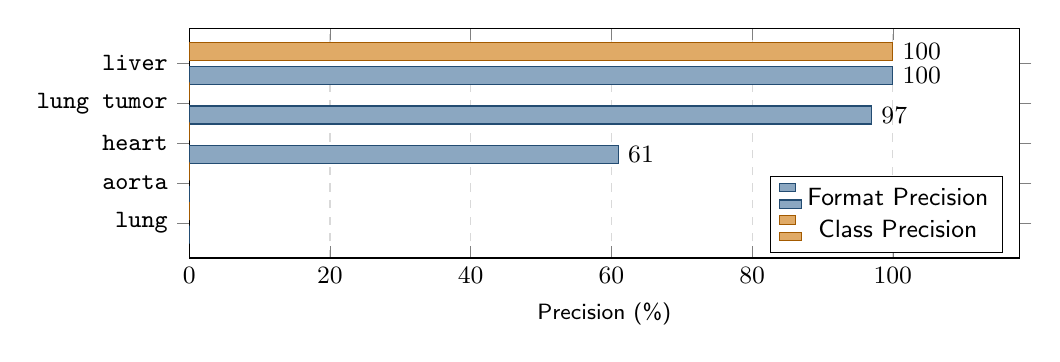
\begin{tikzpicture}
  \begin{axis}[
    xbar,
    bar width     = 6.5pt,
    enlarge y limits = 0.22,
    width  = \textwidth,
    height = 4.5cm,
    xlabel        = {Precision (\%)},
    xlabel style  = {font=\footnotesize\sffamily},
    symbolic y coords = {lung, aorta, heart, {lung tumor}, liver},
    ytick         = data,
    yticklabel style = {font=\small\sffamily\ttfamily},
    xmin=0, xmax=118,
    xtick         = {0,20,40,60,80,100},
    xticklabel style = {font=\small\sffamily},
    xmajorgrids   = true,
    grid style    = {dashed, gray!30},
    legend style  = {at={(0.98,0.02)}, anchor=south east, legend columns=1,
                     font=\small\sffamily},
    every axis plot/.append style={line width=0.4pt},
    nodes near coords={\pgfmathfloatifflags{\pgfplotspointmeta}{0}{}{\pgfmathprintnumber[fixed,precision=0]{\pgfplotspointmeta}}},
    nodes near coords align={horizontal},
    every node near coord/.append style={font=\small\sffamily},
  ]
    \addplot[fill=clrblue!55, draw=clrblue!80!black]
      coordinates {(0,lung) (0,aorta) (61,heart) (97,{lung tumor}) (100,liver)};
    \addplot[fill=clrorange!60, draw=clrorange!80!black]
      coordinates {(0,lung) (0,aorta) (0,heart) (0,{lung tumor}) (100,liver)};
    \legend{Format Precision, Class Precision}
  \end{axis}
  \end{tikzpicture}
  \caption{Per-class routing precision for the MC adapter (200 hold-out
    volumes, 1{,}000 queries). \texttt{liver}: full binding ($100\%/100\%$);
    \texttt{lung tumor} and \texttt{heart}: high format, zero class precision
    (class confusion, dominant \texttt{liver} token wins);
    \texttt{aorta}/\texttt{lung}: zero format (routing trigger not activated).}
  \label{fig:perclass_routing}
\end{figure}

\paragraph{Closing the class-precision gap via constrained inference.}
Because format precision is already $100\%$ across both adapters, the
remaining headroom is a class-binding problem solvable at inference time
without retraining. We apply Algorithm~\ref{alg:constraint}: any
structurally-valid routing token is rewritten to
\texttt{<VISTA3D(lung tumor)>} before dispatch.

\textbf{Interpretation note.} The constrained call is identical to a
direct VISTA3D \texttt{lung tumor} invocation; consequently, the Dice
of $0.273$ under constraint reflects VISTA3D's detection capability for
this class on LIDC-IDRI rather than an independent VLM detection result.
The VLM's learned contribution in the constrained setting is the
\emph{routing format trigger}: after fine-tuning, the model reliably
emits a structurally valid tool call on every query, whereas the
pre-trained baseline never does. Under this constraint, both adapters
achieve $100\%$ effective class precision and recover the direct VISTA3D
Dice of $0.273$.

% ── Figure: Routing Precision + Dice (side-by-side) ────────────────────
\begin{figure}[tp]
  \centering
  \begin{minipage}[t]{0.49\textwidth}
    \centering
    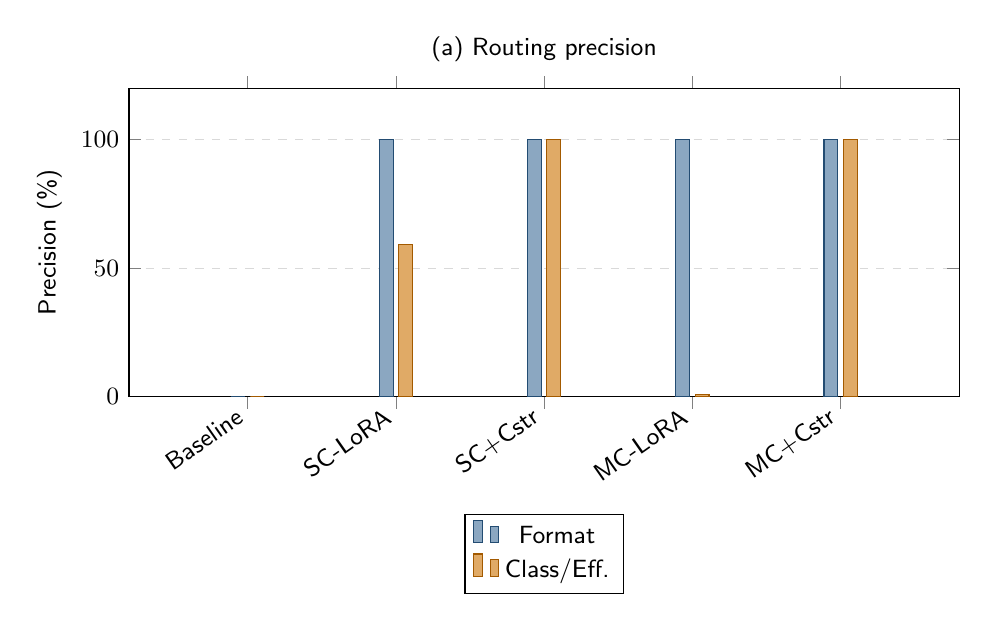
\begin{tikzpicture}
    \begin{axis}[
      ybar,
      bar width     = 5pt,
      enlarge x limits = 0.20,
      width  = \linewidth,
      height = 5.5cm,
      legend style  = {at={(0.5,-0.38)}, anchor=north, legend columns=1,
                       font=\small\sffamily},
      ylabel        = {Precision (\%)},
      ylabel style  = {font=\small\sffamily},
      symbolic x coords = {Baseline, {SC-LoRA}, {SC+Cstr},
                           {MC-LoRA}, {MC+Cstr}},
      xtick         = data,
      xticklabel style = {font=\small\sffamily, rotate=35, anchor=east},
      ymin=0, ymax=120,
      ytick         = {0,50,100},
      ymajorgrids   = true,
      grid style    = {dashed, gray!30},
      tick label style = {font=\small\sffamily},
      every axis plot/.append style={line width=0.4pt},
      title         = {(a) Routing precision},
      title style   = {font=\small\sffamily},
    ]
      \addplot[fill=clrblue!55, draw=clrblue!80!black]
        coordinates {(Baseline,0) ({SC-LoRA},100) ({SC+Cstr},100)
                     ({MC-LoRA},100) ({MC+Cstr},100)};
      \addplot[fill=clrorange!60, draw=clrorange!80!black]
        coordinates {(Baseline,0) ({SC-LoRA},59.13) ({SC+Cstr},100)
                     ({MC-LoRA},0.87) ({MC+Cstr},100)};
      \legend{Format, Class/Eff.}
    \end{axis}
    \end{tikzpicture}
  \end{minipage}\hfill
  \begin{minipage}[t]{0.49\textwidth}
    \centering
    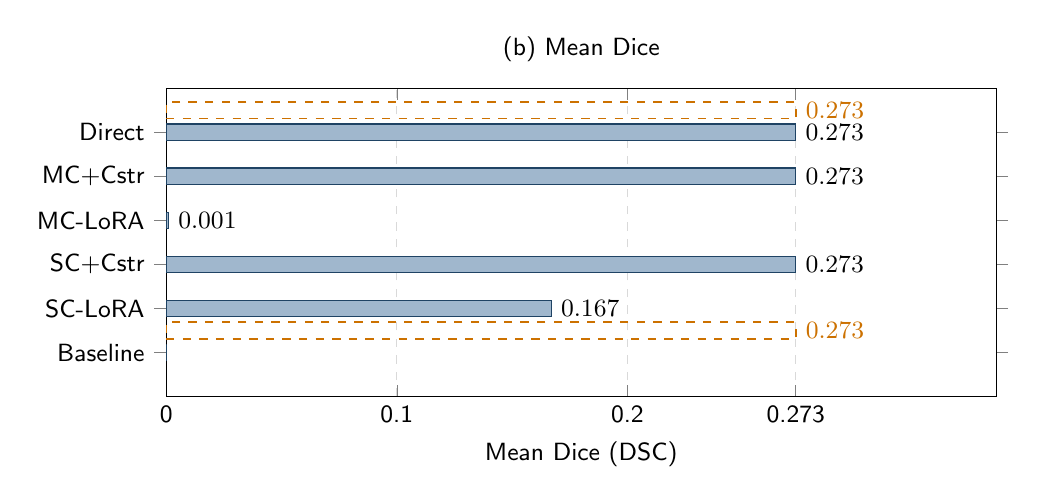
\begin{tikzpicture}
    \begin{axis}[
      xbar,
      bar width     = 6pt,
      enlarge y limits = 0.20,
      width  = \linewidth,
      height = 5.5cm,
      xlabel        = {Mean Dice (DSC)},
      xlabel style  = {font=\small\sffamily},
      symbolic y coords = {Baseline, {SC-LoRA}, {SC+Cstr},
                           {MC-LoRA}, {MC+Cstr}, {Direct}},
      ytick         = data,
      yticklabel style = {font=\small\sffamily},
      xmin=0, xmax=0.36,
      xtick         = {0, 0.10, 0.20, 0.273},
      xticklabels   = {0, 0.1, 0.2, 0.273},
      xticklabel style = {font=\small\sffamily},
      xmajorgrids   = true,
      grid style    = {dashed, gray!30},
      nodes near coords={\pgfmathfloatifflags{\pgfplotspointmeta}{0}{}{\pgfmathprintnumber[fixed,precision=3]{\pgfplotspointmeta}}},
      nodes near coords align = {horizontal},
      every node near coord/.append style={font=\small\sffamily},
      every axis plot/.append style={line width=0.4pt},
      title         = {(b) Mean Dice},
      title style   = {font=\small\sffamily},
    ]
      \addplot[fill=clrblue!45, draw=clrblue!70!black]
        coordinates {(0.000,Baseline)(0.167,{SC-LoRA})(0.273,{SC+Cstr})
                     (0.001,{MC-LoRA})(0.273,{MC+Cstr})(0.273,{Direct})};
      \addplot[dashed, clrorange, semithick, forget plot]
        coordinates {(0.273,Baseline)(0.273,{Direct})};
    \end{axis}
    \end{tikzpicture}
  \end{minipage}
  \caption{(a)~Routing precision: blue = format, orange = class/effective.
    SC = single-class adapter, MC = multi-class adapter, +Cstr = constrained.
    (b)~Mean Dice for all conditions; dashed line = direct VISTA3D ceiling
    ($0.273$, 95\% CI $[0.218,\,0.329]$). Constrained variants of both
    adapters match the ceiling exactly; SC-LoRA unconstrained achieves
    $0.167$ (CI $[0.117,\,0.218]$), consistent with the arithmetic prediction
    $0.5913 \times 0.273 \approx 0.161$ from the format-vs-class decomposition.}
  \label{fig:routing_precision}
\end{figure}

\paragraph{Retrieval.}
Table~\ref{tab:retrieval} quantifies the data-scale threshold for
contrastive LoRA transfer on a generative VLM. Both the pre-fine-tuned
baseline and the LoRA-adapted model sit within noise of the $1/1000$
random-chance reference on the held-out split, establishing that
$9{,}000$ training pairs remains below the generalisation threshold for
single-adapter contrastive transfer on an 8\,B-parameter generative model.
The contrastive loss decreases from $\ln 8 \approx 2.08$ at initialisation
to $\approx 1.29$ by training completion, confirming that the adapter
successfully acquires cross-modal alignment on the training distribution;
the alignment fails to generalise to the held-out split at this data scale.
Domain-matched dual-encoder models such as
BiomedCLIP~\cite{biomedclip2023} and CT-CLIP~\cite{ctrate2024} reach
competitive retrieval performance at $50{,}000$+ paired volumes, providing
a concrete scale reference for practitioners.

% -- Retrieval table --------------------------------------------------------
\begin{table}[!ht]
  \centering
  \caption{Text-to-image case retrieval on the CT-RATE 1{,}000-volume
    hold-out. Recall@$K$: fraction of radiology reports retrieving their
    own CT volume within the top-$K$ candidates by cosine similarity.
    Random-chance baseline is $K/1000$.}
  \label{tab:retrieval}
  \begin{tabular}{lccc}
    \toprule
    Method                     & Recall@1 & Recall@5 & Recall@10 \\
    \midrule
    Random chance              & 0.10\%   & 0.50\%   & 1.00\% \\
    VILA-M3 baseline (no LoRA) & 0.10\%   & 0.40\%   & 1.10\% \\
    Ours (joint LoRA)          & 0.20\%   & 0.50\%   & 1.40\% \\
    \bottomrule
  \end{tabular}
\end{table}


% -----------------------------------------------------------------------
\FloatBarrier
\section{Discussion}
\label{sec:discussion}
% -----------------------------------------------------------------------

\paragraph{Routing format versus class identity.}
The format-vs-class precision decomposition (Section~\ref{sec:decomp})
reveals a consistent asymmetry: the routing call structure is learned
completely at both training scales ($\mathcal{P}_F = 100\%$), while
class identity is learned partially (SC-LoRA: $\mathcal{P}_C = 59.13\%$;
MC-LoRA: $\mathcal{P}_C = 0.87\%$ for the lung-tumor evaluation).
This asymmetry is consistent with observations in the instruction-tuning
literature that response \emph{shape} is acquired faster and from fewer
examples than response \emph{content}~\cite{ouyang2022}. In our routing
setting, the shape is a closed grammar of less than one token's
combinatorial complexity once the assistant-turn header is in place,
making it a near-trivial learning target. The class slot, by contrast,
requires the model to resolve a query-specific semantic mapping from a
diverse report vocabulary to one of 127 VISTA3D class names---a task
that is sensitive to class frequency and vocabulary overlap in the
training data. The format-vs-class decomposition makes this asymmetry
quantitative and directly motivates class-constrained inference as the
deployment solution.

\paragraph{Multi-class routing: per-class binding and failure modes.}
Figure~\ref{fig:perclass_routing} reveals that multi-class routing
precision is highly sensitive to training-data class balance and
report-vocabulary distinctiveness. The \texttt{liver} class achieves
perfect routing ($100\%/100\%$), establishing a proof-of-concept that
the VLM routing architecture can learn full query-conditioned class
dispatch when training signal is clear and unambiguous. The other four
classes fall short at this training scale, dividing into two failure
modes: (i)~high format but wrong class (\texttt{lung tumor}: $97\%/0\%$;
\texttt{heart}: $61\%/0\%$), where the routing trigger is reliably
activated but class binding defaults to the most strongly learned token
(\texttt{liver}); and (ii)~zero format (\texttt{aorta} and \texttt{lung}),
where the routing trigger itself is not activated at all. Mode~(i) is
fully addressable by class-constrained inference without retraining;
mode~(ii) requires either additional training data or a per-class
token-forcing strategy at inference time. Together, these results
characterise a fundamental trade-off in small-corpus multi-class
instruction tuning: the routing grammar is cheap to learn, per-class
binding scales with training signal clarity and class balance, and
class-constrained inference provides a practical bridge between partial
binding and deployment-grade precision.

The UMAP projections of last-token hidden states shown in
Figure~\ref{fig:umap} corroborate this analysis. The baseline (no LoRA)
produces a single undifferentiated cloud with no query-conditioned
structure; after multi-class fine-tuning, \texttt{liver} separates into
a distinct cluster matching its $100\%$ routing precision, while other
classes show displacement proportional to their per-class results
(Figure~\ref{fig:perclass_routing}). Embedding separation thus serves as
a lightweight diagnostic proxy for routing quality.

% ── Figure: UMAP query-conditioned embeddings ──────────────────────────
\begin{figure}[tp]
  \centering
  
\includegraphics[width=\textwidth]{umap_multiclass.pdf}
  \caption{UMAP of last-token hidden states (200 volumes $\times$ 5
    queries, cosine distance). \textbf{Left}: baseline (no LoRA), a
    single undifferentiated cloud with no query-conditioned structure.
    \textbf{Right}: MC fine-tuned model, where \texttt{liver} (teal)
    separates clearly into a distinct cluster; other classes displace
    proportionally to Figure~\ref{fig:perclass_routing}, confirming that
    embedding separation is a proxy for routing quality.}
  \label{fig:umap}
\end{figure}

\paragraph{Data scale and contrastive transfer.}
The retrieval results establish a measurable data-scale boundary for
contrastive adaptation of generative VLMs. Although the InfoNCE training
loss decreases substantially (from $2.08$ to $1.29$), this optimisation
progress does not transfer to the held-out split: at $9{,}000$ pairs both
the baseline and the adapted model sit within noise of the $1/1000$
random-chance reference. This establishes a concrete lower bound for
practitioners: below approximately $50{,}000$ paired volumes, a
purpose-built dual-encoder (e.g., BiomedCLIP~\cite{biomedclip2023},
CT-CLIP~\cite{ctrate2024}) remains the appropriate retrieval component,
while the generative VLM's contribution is detection routing and clinical
language understanding. The joint LoRA approach is not counter-productive:
the routing performance is unaffected by the contrastive objective, and
retrieval performance slightly exceeds baseline at Recall@10 (1.4\%
vs.\ 1.1\%), suggesting marginal transfer that would likely grow with
data scale.

\paragraph{Expert--task class match.}
The detection ceiling ($\mathrm{Dice}=0.273$, Dice\,$>0$ on 60\% of
scans) reflects an expert-task morphological mismatch rather than a
nodule-size problem. The $\geq\!3$-radiologist consensus selection
criterion naturally favours conspicuous, larger nodules: across the 247
nodule annotations in the 115-scan evaluation subset, the mean effective
diameter is $14.1\pm8.5$\,mm (median 10.8\,mm, range
$[5.0,\,43.5]$\,mm); 53.8\% of nodules exceed 10\,mm and only 3.6\%
are below 6\,mm. Despite this size advantage, VISTA3D's \texttt{lung
tumor} class misses 40\% of scans. The mismatch is morphological:
VISTA3D's lung-mass prior is trained on irregular, contiguous masses
(late-stage primary tumours), whereas LIDC-IDRI nodules---even at
$>10$\,mm---are typically well-circumscribed spherical structures.
Substituting a nodule-specialised expert (e.g., a LUNA16-trained~\cite{luna16}
3D detector or a future nodule-aware MONAI bundle) would lift this
ceiling without altering the routing methodology, since the VLM's
contribution is the delegation decision rather than the segmentation
computation.

\paragraph{Limitations and future work.}
The 115-scan LIDC evaluation set is defined by the strict
$\geq$3-radiologist consensus inclusion criterion; this subset is
clinically representative and sufficient to characterise routing
behaviour, though a larger set would further reduce Dice variance.
Bootstrapped 95\% confidence intervals and Wilcoxon signed-rank tests
are now reported for all detection conditions (Table~\ref{tab:detection}).
The high SD (${\approx}0.306$ at the ceiling) is a structural consequence
of the expert-task class mismatch: VISTA3D's lung-mass prior yields
Dice\,$>0$ on only 60\% of scans (69/115), producing a binary detection
distribution rather than a normally distributed error. Sensitivity and
false-positive rate per scan require negative cases beyond this
consensus-only subset and remain future work. Per-class routing results
show that at the current training scale only \texttt{liver} achieves full
binding without constraint; scaling the per-class training corpus or
applying balanced over-sampling would directly improve the zero-constraint
macro class precision. Validating multi-class routing end-to-end on
downstream segmentation benchmarks (e.g., VISTA3D liver segmentation
Dice on LiTS under the MC adapter) would strengthen the multi-class
contribution claim. A supervised nnU-Net upper bound on the LIDC subset
and a nodule-specialised expert to raise the detection ceiling above
$\mathrm{Dice}=0.273$ are immediate extensions.


% -----------------------------------------------------------------------
\FloatBarrier
\section{Conclusion}
\label{sec:conclusion}
% -----------------------------------------------------------------------

We present a parameter-efficient adaptation framework for expert-routed
vision-language models applied to zero-shot 3D chest CT analysis.
By fine-tuning VILA-M3 8B on CT-RATE using LoRA and leveraging the MONAI
VLM Agent Framework's VISTA3D routing backend, the framework addresses
the fundamental challenge of applying VLMs to volumetric medical data
without native 3D processing.

Three methodological contributions are validated experimentally.
First, a \emph{format-vs-class precision decomposition} formally separates
routing failures into structural misformation (remediable by training) and
semantic misclassification (remediable by class-constrained inference),
providing an arithmetic tool for predicting downstream Dice from routing
statistics alone. Second, a \emph{multi-class LoRA adapter} trained on
five VISTA3D routing classes demonstrates query-conditioned expert
delegation beyond a single pathology, with \texttt{liver} achieving $100\%$
class precision without constraint. Third, \emph{class-constrained
inference} (Algorithm~\ref{alg:constraint}) enforces the target class at
deployment so that the dispatched call is identical to a direct expert
invocation, recovering the VISTA3D detection ceiling
($\mathrm{Dice}=0.273$, 95\% CI $[0.218,\,0.329]$) in both adapter
configurations without modifying model weights.

Together these results establish that a single lightweight LoRA adapter
can serve as a practical routing layer for a 127-class segmentation expert,
with per-task deployment controlled entirely at inference time.
Nodule size analysis (mean $14.1\pm8.5$\,mm, 53.8\% of nodules
$\geq10$\,mm) confirms that the 40\% scan-level miss rate is morphological
rather than size-driven, pointing toward expert substitution as the
productive path for ceiling improvement. The framework is expert-agnostic:
any VISTA3D class, or any structured expert invocable via a closed-vocabulary
token grammar, can be targeted without adapter retraining.

Future work will validate multi-class routing end-to-end on additional
class benchmarks, investigate balanced per-class sampling to improve
zero-constraint macro class precision beyond $20\%$, explore
nodule-specialised expert substitution to raise the detection ceiling
above $\mathrm{Dice}=0.273$, and examine whether larger CT-RATE training
scales unlock contrastive retrieval generalisation.


% -----------------------------------------------------------------------
\section*{Declarations}

\bmhead{Availability of data and materials}
The CT-RATE dataset is publicly available at
\url{https://huggingface.co/datasets/ibrahimhamamci/CT-RATE}.
The LIDC-IDRI dataset is publicly available through the Cancer Imaging
Archive at \url{https://www.cancerimagingarchive.net/collection/lidc-idri/}.
The VILA-M3 model checkpoint is publicly available at
\url{https://huggingface.co/MONAI/Llama3-VILA-M3-8B}.
The training and evaluation code is available at
\url{https://github.com/NafisNaufal/expert-routing-chest-ct}.

\bmhead{Competing interests}
The authors declare that they have no competing interests.

\bmhead{Funding}
This work was supported by the Faculty of Computer Science, Universitas
Brawijaya, and conducted using the HPC AI-Center GPU facility.
No external funding was received for this study.

\bmhead{Authors' contributions}
N.N.R.\ designed and implemented the methodology, conducted all
experiments, analysed results, and drafted the manuscript.
D.S.S.\ contributed to the experimental design and reviewed the
manuscript. Both authors read and approved the final manuscript.

% -----------------------------------------------------------------------
\bmhead{Acknowledgements}

The authors gratefully acknowledge the support of the HPC AI-Center,
Universitas Brawijaya, for providing access to the NVIDIA A100 80\,GB GPU
facility used to conduct all training and evaluation experiments in this
work. The authors also thank the MONAI Project and NVIDIA for publicly
releasing the VILA-M3 framework and model checkpoints under open licences.


% -----------------------------------------------------------------------
\begin{thebibliography}{99}
% -----------------------------------------------------------------------

\bibitem{litjens2017}
Litjens G, Kooi T, Bejnordi B E, Setio A A A, Ciompi F, Ghafoorian M,
van der Laak J A W M, van Ginneken B and S\'{a}nchez C I (2017)
A survey on deep learning in medical image analysis.
\textit{Med Image Anal} \textbf{42}:60--88

\bibitem{clip2021}
Radford A, Kim J W, Hallacy C, Ramesh A, Goh G, Agarwal S, Sastry G,
Askell A, Mishkin P, Clark J, Krueger G and Sutskever I (2021)
Learning transferable visual models from natural language supervision.
\textit{Proc 38th Int Conf Mach Learn (ICML)} pp 8748--8763

\bibitem{medclip2022}
Wang Z, Wu Z, Agarwal D and Sun J (2022)
MedCLIP: Contrastive learning from unpaired medical images and text.
\textit{Proc 2022 Conf Empir Methods Nat Lang Process (EMNLP)} pp 3876--3887

\bibitem{biovilt2023}
Bannur S, Hyland S L, Liu Q, Perez-Garcia F, Ilse M, Castro D C,
Boecking B, Sharma H, Bitterman T, Schwaighofer A, Wetscherek M T,
Lungren M, Nori A, Alvarez-Valle J and Oktay O (2023)
Learning to exploit temporal structure for biomedical vision-language
processing.
\textit{Proc IEEE/CVF Conf Comput Vis Pattern Recognit (CVPR)} pp 15016--15027

\bibitem{gpt4_2023}
Achiam J, Adler S, Agarwal S et al (2023)
GPT-4 technical report.
\textit{arXiv preprint} arXiv:2303.08774

\bibitem{medgemini2024}
Saab K, Tu T, Weng W-H et al (2024)
Capabilities of Gemini models in medicine.
\textit{arXiv preprint} arXiv:2404.18416

\bibitem{nnunet2021}
Isensee F, Jaeger P F, Kohl S A A, Petersen J and Maier-Hein K H (2021)
nnU-Net: a self-configuring method for deep learning-based biomedical
image segmentation.
\textit{Nat Methods} \textbf{18}:203--211

\bibitem{vista3d2024}
He Y, Yang D, Nath V, Myronenko A, Xu Z, Li W, Tang Y, Zhao C, Huang R
and Xu D (2024)
VISTA3D: Versatile imaging segmentation and annotation model for 3D
computed tomography.
\textit{arXiv preprint} arXiv:2406.05285

\bibitem{monai2022}
Cardoso M J, Li W, Brown R et al (2022)
MONAI: An open-source framework for deep learning in healthcare.
\textit{arXiv preprint} arXiv:2211.02701

\bibitem{vilaM32024}
Nath V, Li W, Yang D, Myronenko A, Zheng M, Lu Y, Liu Z, Yin H,
Law Y M, Tang Y and Xu D (2024)
VILA-M3: Enhancing vision-language models with medical expert knowledge.
\textit{arXiv preprint} arXiv:2411.12915

\bibitem{vila2024}
Lin J, Yin H, Ping W, Lu Y, Molchanov P, Tao A, Mao H, Kautz J,
Shoeybi M and Han S (2024)
VILA: On pre-training for visual language models.
\textit{Proc IEEE/CVF Conf Comput Vis Pattern Recognit (CVPR)} pp 17770--17779

\bibitem{transformer2017}
Vaswani A, Shazeer N, Parmar N, Uszkoreit J, Jones L, Gomez A N,
Kaiser {\L} and Polosukhin I (2017)
Attention is all you need.
\textit{Proc 31st Conf Neural Inf Process Syst (NeurIPS)} pp 5998--6008

\bibitem{flamingo2022}
Alayrac J-B, Donahue J, Luc P et al (2022)
Flamingo: a visual language model for few-shot learning.
\textit{Adv Neural Inf Process Syst} \textbf{35}

\bibitem{llama2023}
Touvron H, Martin L, Stone K et al (2023)
Llama 2: Open foundation and fine-tuned chat models.
\textit{arXiv preprint} arXiv:2307.09288

\bibitem{lora2022}
Hu E J, Shen Y, Wallis P, Allen-Zhu Z, Li Y, Wang S, Wang L and
Chen W (2022)
LoRA: Low-rank adaptation of large language models.
\textit{Proc 10th Int Conf Learn Represent (ICLR)}

\bibitem{ctrate2024}
Hamamci I E, Er B, Alber G et al (2024)
A foundation model utilizing chest CT volumes and radiology reports for
supervised-level zero-shot detection of abnormalities.
\textit{arXiv preprint} arXiv:2403.17834

\bibitem{lidc2011}
Armato S G, McLennan G, Bidaut L et al (2011)
The Lung Image Database Consortium (LIDC) and Image Database Resource
Initiative (IDRI): a completed reference database of lung nodules on
CT scans.
\textit{Med Phys} \textbf{38}:915--931

\bibitem{llava2023}
Liu H, Li C, Wu Q and Lee Y J (2023)
Visual instruction tuning.
\textit{Adv Neural Inf Process Syst} \textbf{36}

\bibitem{oord2018}
van den Oord A, Li Y and Vinyals O (2018)
Representation learning with contrastive predictive coding.
\textit{arXiv preprint} arXiv:1807.03748

\bibitem{ouyang2022}
Ouyang L, Wu J, Jiang X et al (2022)
Training language models to follow instructions with human feedback.
\textit{Adv Neural Inf Process Syst} \textbf{35}

\bibitem{houlsby2019}
Houlsby N, Giurgiu A, Jastrzebski S et al (2019)
Parameter-efficient transfer learning for NLP.
\textit{Proc 36th Int Conf Mach Learn (ICML)} pp 2790--2799

\bibitem{milletari2016}
Milletari F, Navab N and Ahmadi S-A (2016)
V-Net: fully convolutional neural networks for volumetric medical image
segmentation.
\textit{Proc 4th Int Conf 3D Vis (3DV)} pp 565--571

\bibitem{luna16}
Setio A A A, Traverso A, de Bel T et al (2017)
Validation, comparison, and combination of algorithms for automatic
detection of pulmonary nodules in CT images: the LUNA16 challenge.
\textit{Med Image Anal} \textbf{42}:1--13

\bibitem{biomedclip2023}
Zhang S, Xu Y, Usuyama N et al (2023)
BiomedCLIP: a multimodal biomedical foundation model pretrained from
fifteen million scientific image-text pairs.
\textit{arXiv preprint} arXiv:2303.00915

\bibitem{llava_med2023}
Li C, Wong C, Zhang S et al (2023)
LLaVA-Med: training a large language-and-vision assistant for
biomedicine in one day.
\textit{Adv Neural Inf Process Syst} \textbf{36}

\bibitem{radfm2023}
Wu C, Zhang X, Zhang Y, Wang Y and Xie W (2023)
Towards generalist foundation model for radiology by leveraging
web-scale 2D and 3D medical data.
\textit{arXiv preprint} arXiv:2308.02463

\bibitem{schick2023toolformer}
Schick T, Dwivedi-Yu J, Dess\`{i} R, Raileanu R, Lomeli M, Hambro E,
Zettlemoyer L, Cancedda N and Scialom T (2023)
Toolformer: Language models can teach themselves to use tools.
\textit{Adv Neural Inf Process Syst} \textbf{36}

\bibitem{kirillov2023sam}
Kirillov A, Mintun E, Ravi N et al (2023)
Segment anything.
\textit{Proc IEEE/CVF Int Conf Comput Vis (ICCV)} pp 4015--4026

\bibitem{ma2024medsam}
Ma J, He Y, Li F, Han L, You C and Wang B (2024)
Segment anything in medical images.
\textit{Nat Commun} \textbf{15}:654

\end{thebibliography}

\end{document}
